% arara: xelatex
% arara: biber
% arara: xelatex
% arara: xelatex
%%% arara: clean: { files: [riemann_main.log,riemann_main.aux,riemann_main.blg,riemann_main.bbl,riemann_main.bcf,riemann_main.toc,riemann_main.run.xml] }
%%% arara: lmkclean
%%% arara: pdflatex
%%% arara: pdflatex
%%% % arara: lmkclean
%%% zsh> setopt no_nomatch

% Chandra Images by Category: Supernovas & Supernova Remnants
% https://chandra.harvard.edu/photo/category/snr.html

\documentclass[a4paper,12pt]{extarticle}

\RequirePackage[l2tabu,orthodox]{nag} % Раскомментировав, можно в логе получать рекомендации относительно правильного использования пакетов и предупреждения об устаревших и нерекомендуемых пакетах
% \documentclass[a4paper,14pt]{extarticle}
\usepackage[left=1.5 cm,right=1.6cm,top=1.5cm,bottom=2.5cm]{geometry}

%%% Mathematical packages %%%
\usepackage{amsthm,amsmath,amscd} % Математические дополнения от AMS
\usepackage{amsfonts,amssymb}     % Математические дополнения от AMS
\usepackage{mathtools}            % Добавляет окружение multlined
\usepackage{mathtext}
\usepackage{cancel}

\usepackage{textcomp}

\RequirePackage{ifxetex, ifluatex}
\ifxetex
  % https://tex.stackexchange.com/a/38631
  \renewcommand{\mathbf}{\ensuremath{\symbf}}
  \usepackage{unicode-math}
  \usepackage{polyglossia}                        % Поддержка многоязычности (fontspec подгружается автоматически)
 % \setmainlanguage[babelshorthands=true]{russian} % Язык по-умолчанию русский с поддержкой приятных команд пакета babel
  \setotherlanguage{english}                      % Дополнительный язык = английский (в американской вариации по-умолчанию)
  % Семейство шрифтов Liberation (https://pagure.io/liberation-fonts)
  \setmonofont{LiberationMono}[Scale=0.87]        % моноширинный шрифт
  \newfontfamily\cyrillicfonttt{LiberationMono}[  % моноширинный шрифт для кириллицы
    Scale=0.87]
  \defaultfontfeatures{Ligatures=TeX}             % стандартные лигатуры TeX, замены нескольких дефисов на тире и т. п. Настройки моноширинного шрифта должны идти до этой строки, чтобы при врезках кода программ в коде не применялись лигатуры и замены дефисов
  \setmainfont{LiberationSerif}                   % Шрифт с засечками
  \newfontfamily\cyrillicfont{LiberationSerif}    % Шрифт с засечками для кириллицы
  \setsansfont{LiberationSans}                    % Шрифт без засечек
  \newfontfamily\cyrillicfontsf{LiberationSans}   % Шрифт без засечек для кириллицы

  % fake small capitals
  % https://tex.stackexchange.com/questions/55664/fake-small-caps-with-xetex-fontspec
  \makeatletter
  \newlength\fake@f
  \newlength\fake@c
  \def\textsc#1{%
    \begingroup%
    \xdef\fake@name{\csname\curr@fontshape/\f@size\endcsname}%
    \fontsize{\fontdimen8\fake@name}{\baselineskip}\selectfont%
    \MakeUppercase{#1}%
    \endgroup%
    }
  \makeatother
  % \renewcommand{\textsc}[1]{\fauxschelper#1 \relax\relax}
  % \def\fauxschelper#1 #2\relax{%
  %   \fauxschelphelp#1\relax\relax%
  %   \if\relax#2\relax\else\ \fauxschelper#2\relax\fi%
  %   }
  % \def\Hscale{.83}\def\Vscale{.72}\def\Cscale{1.00}
  % \def\fauxschelphelp#1#2\relax{%
  %   \ifnum`#1>``\ifnum`#1<`\{\scalebox{\Hscale}[\Vscale]{\uppercase{#1}}\else%
  %   \scalebox{\Cscale}[1]{#1}\fi\else\scalebox{\Cscale}[1]{#1}\fi%
  %   \ifx\relax#2\relax\else\fauxschelphelp#2\relax\fi}

\else
  \usepackage[T2A]{fontenc}           % кодировка
  \usepackage[utf8]{inputenc}         % Кодировка utf8
  \usepackage[english,russian]{babel} % Языки: русский, английский
\fi

\usepackage[colorlinks=true,unicode=true]{hyperref}

%%% Other packages %%%
\usepackage{xspace} % пробелы после предопределённых команд
\usepackage{color}
\usepackage{enumitem}
\usepackage{cmap}
\usepackage{array}
\usepackage{braket}
\usepackage{epsfig}
\usepackage{epstopdf}
\usepackage{graphicx}
\usepackage{float}
\usepackage{caption}
\captionsetup{compatibility=false}
\usepackage{subcaption}
\usepackage{indentfirst}
\usepackage{hyphenat}
\usepackage[normalem]{ulem}
\usepackage{wrapfig}
\usepackage{pdfpages}

\graphicspath{{img/}} % Пути к изображениям

%%% Toc %%%
% \setcounter{tocdepth}{4}
% \setcounter{secnumdepth}{4}

%%% Title %%%
% \usepackage{titlesec}
% \titleformat{\section}
% {\normalfont\large\bfseries}{\thesection}{1em}{}

%%% Setup bibliography %%%

\usepackage{csquotes} % biblatex рекомендует его подключать. Пакет для оформления сложных блоков цитирования.
%%% Загрузка пакета с основными настройками %%%
\makeatletter
\usepackage[%
backend=biber,% движок
bibencoding=utf8,% кодировка bib файла
sorting=none,% настройка сортировки списка литературы
style=gost-numeric,% стиль цитирования и библиографии (по ГОСТ)
language=autobib,% получение языка из babel/polyglossia, default: autobib % если ставить autocite или auto, то цитаты в тексте с указанием страницы, получат указание страницы на языке оригинала
autolang=other,% многоязычная библиография
clearlang=true,% внутренний сброс поля language, если он совпадает с языком из babel/polyglossia
defernumbers=true,% нумерация проставляется после двух компиляций, зато позволяет выцеплять библиографию по ключевым словам и нумеровать не из большего списка
sortcites=true,% сортировать номера затекстовых ссылок при цитировании (если в квадратных скобках несколько ссылок, то отображаться будут отсортированно, а не абы как)
movenames=false, % опция разрешает или запрещает перемещение имён в область сведений об ответственности, если количество имён больше трёх.
% не менять местами заголовок и список авторов, если авторов больше четырех
minnames=3, % сокращение списка имён
maxnames=4, % сокращение списка имён
doi=true,% Показывать или нет ссылки на DOI
isbn=false,% Показывать или нет ISBN, ISSN, ISRN
url=false,
eprint=true,
backref=true
]{biblatex}[2016/09/17]
%]{biblatex}
%\ltx@iffilelater{biblatex-gost.def}{2017/05/03}%
{\toggletrue{bbx:gostbibliography}%
\renewcommand*{\revsdnamepunct}{\addcomma}}{}
\makeatother

\DefineBibliographyStrings{english}{docthesis = {dissertation}}
\DefineBibliographyStrings{russian}{docthesis = {диссертация}}

% Custom backref Text
%https://tex.stackexchange.com/questions/196015/custom-backref-text
\DefineBibliographyStrings{english}{
  backrefpage  = {Цит. на с.\adddot},
  backrefpages = {Цит. на с.\adddot},
}
\DefineBibliographyStrings{russian}{
  backrefpage  = {Цит. на с.\adddot},
  backrefpages = {Цит. на с.\adddot},
}
\ifxetex
\else
% Исправление случая неподдержки знака номера в pdflatex
    \DefineBibliographyStrings{russian}{number={\textnumero}}
\fi

% разделитель ; для ссылок
\DeclareMultiCiteCommand{\multicites}[\mkbibbrackets]{\cite}{\addsemicolon\space}

%%% Colors %%%
\usepackage[dvipsnames]{xcolor}

\definecolor{linkcolor}{rgb}{0.08, 0.38, 0.74}
\definecolor{citecolor}{rgb}{0.18, 0.55, 0.34}
\definecolor{urlcolor}{rgb}{0.03, 0.57, 0.82}

\hypersetup{
    linktocpage=true,           % ссылки с номера страницы в оглавлении, списке таблиц и списке рисунков
    colorlinks,                 % ссылки отображаются раскрашенным текстом, а не раскрашенным прямоугольником, вокруг текста
    linkcolor={linkcolor},      % цвет ссылок типа ref, eqref и подобных
    citecolor={citecolor},      % цвет ссылок-цитат
    urlcolor={urlcolor},        % цвет гиперссылок
}

%%% Users commands %%%

\def\stella{\code{STEL\-LA}\xspace}
\def\millimetron{\code{Миллиметрон}\xspace}
\def\mesa{\code{ME\-SA}\xspace}
\def\supremna{\code{SUP\-REM\-NA}\xspace}

\def\araa{Annual Review of Astronomy and Astrophysics}
\def\apj{The Astrophysical Journal}
\def\apjl{The Astrophysical Journal Letters}
\def\apjs{The Astrophysical Journal Supplement}
\def\apss{Astrophysics and Space Science}
\def\azh{Астрон. Журнал}
\def\pazh{Письма в Астрон. Журнал}
\def\pasp{Pub. Astron. Soc. Pacific}
\def\pasa{Pub. Astron. Soc. Australia}
\def\prl{Phys. Rev. Lett}
\def\pre{Phys. Rev. E}
\def\sovast{Soviet Astronomy}
\def\aa{Astronomy and Astrophysics}
\def\aapr{Astronomy and Astrophysics Reviews}
\def\aj{Astronomical Journal}
\def\mnras{MNRAS}
\def\nat{Nature}
\def\ssr{Space Science Reviews}
\def\prd{Phys. Rev. D}
\def\jqsrt{Journal of Quantitative Spectroscopy and Radiative Transfer}

\DeclareRobustCommand{\todo}{\textcolor{red}}

\newcommand{\code}[1]{\texttt{#1}}
% \newcommand{\code}[1]{\textsc{#1}}
\newcommand\vecx[1]{\ifstrequal{#1}{0}{\ensuremath{\mathbf{0}}}{\ensuremath{\boldsymbol{#1}}}}

\newcommand\vecxu{\vecx{u}}



\newcommand{\pb}[1]{\textbf{\color{magenta}PB: #1}}
\newcommand{\iz}[1]{\textbf{\color{orange}IZ: #1}}

\newcommand\nifsx{$^{56}$Ni\xspace}
\newcommand\cofsx{$^{56}$Co\xspace}
\newcommand\fefsx{$^{56}$Fe\xspace}
\newcommand{\rsun}{\ensuremath{R_\odot}\xspace}
\newcommand{\msun}{\ensuremath{M_\odot}}

% 
\def\rej{\ensuremath{R_{\rm ej}}}
\def\mej{\ensuremath{M_{\rm ej}}}
\def\renv{\ensuremath{R_{\rm env}}}
\def\menv{\ensuremath{M_{\rm env}}}

\newcommand\snia{SN\,Ia\xspace}
\newcommand\snib{SN\,Ib\xspace}
\newcommand\snic{SN\,Ic\xspace}
\newcommand\sniib{SN\,IIb\xspace}
\newcommand\sniip{SN\,IIP\xspace}


\makeatletter
\@ifundefined{c@basement}{
  \newcounter{basement}
  \setcounter{basement}{0} % 0 --- hide basement;
                            % 1 --- show basement
}{}
\makeatother

\hyphenation{
  smooth-ed
  par-tic-le
  hy-dro-dy-nam-ics
}


%%% Add bibliography
\addbibresource{refs_hd_gydro.bib}

\begin{document}

%%% article title
\title{\large
 Заметки про задачу о распаде произвольного разрыва (задача Римана)
}

\author{Илья~Заворохин, П.В.~Бакланов}

\date{\today}

\maketitle

\tableofcontents

%\newpage

%%%%% BEGIN
%------------------------------------------
%\section*{TODO}

%\begin{enumerate}

%\end{enumerate}

%------------------------------------------

\section{Введение}

Цель работы - знакомство с физикой ударных волн, их формирование и эволюция.
Исследовать некоторые частные физические модели, допускающие аналитические решения. 
Получить решения численными методами и сравнить с аналитическими выражениями.
\\

В ограниченной трубе с двумя газами в различных начальных состояниях в начальный момент времени разрывается диафрагма. В последующие моменты времени происходит движение контактного разрыва, а также ударной волны в сторону газа с меньшими давлением и плотностью. При этом в сторону газа с большим давлением распространяется волна разрежения.

%------------------------------------------

\section{Характерные единицы измерения}


%----------------------------
\section{Формулировка задачи Римана}

Рассматривается одномерная задача: 
в момент $t=0$ в трубе находится идеальный газ, разделённый  непроницаемой жёсткой перегородкой. 
Слева от перегородки в области~1 и  справа~2 состояния газа произвольны и независимы друг от друга. 

\todo{Нарисовать и вставить картинку с начальной конфигурацией $t=0$}

Требуется найти состояние газа после того как моментально уберут перегородку. 
Или другими словами, описать как будут меняться от времени свойства газа: формулы, табличный вид, графики. 

Заметки на память можно вставлять с помощью команды:
\begin{verbatim}
	\iz{какой-то текст заметки}
\end{verbatim}
 
Это будет выглядеть так: 	
\iz{какой-то текст заметки}

%----------------------------
\section{Решение задачи Римана}

Выпишем систему уравнений газодинамики, определяющих изменение свойств газа: плотность, скорость и давление \cite{zr1968}.

\begin{align} 
	\frac{\partial \rho}{\partial t} + div(\rho \vecxu) = 0 \label{eq:continuity}\\
	%
	\frac{\partial  \vecxu}{\partial t} + \left(\vecxu \nabla \right)\vecxu = -\frac{1}{\rho}\nabla P  \label{eq:euler}	\\
	%
	\frac{\partial }{\partial t}\rho(E+\frac{\vecxu^2}{2}) + div(\rho \vecxu (w+\frac{\vecxu^2}{2})) = 0  \label{eq:energy} \\
        %
        p = p(\rho,e)
\end{align}
Помимо этого выполнено равенство для энтропии:
    $$ \frac{\partial s}{\partial t} + \vecxu \cdot div(s) = 0 \label{eq:entropy} $$
Показатель адиабаты $\gamma = 1.4$. \\

Выведем соотношения Ранкина--Гюгонио. \\ 
Для этого перепишем данную систему дифференциальных уравнений для данного случая (одномерная трубка),считая что параметры газа претерпевают разрыв на ударной волне.
Обозначив V - скорость ударной волны, получаем:
\begin{align}
    \rho_1V = \rho_2(V-u_2) \mbox{  - закон сохранения потока массы}  \\
    \rho_1V^2 + p_1 = \rho_2(V-u_2)^2 + p_2 \mbox{  - закон сохранения потока импульса} \\
    \frac{V^2}{2}+\frac{\gamma}{\gamma-1}\frac{p_1}{\rho_1} = \frac{(V-u_2)^2}{2}+\frac{\gamma}{\gamma-1}\frac{p_2}{\rho_2} \mbox{  - закон сохранения потока энергии}
\end{align}   
Введя $M = V/c_1$ - число Маха, где $ c_1 =  \frac{\gamma p_1}{\rho_1}$ - скорость в невозмущенной среде справа.
Теперь, проделав некоторые несложные преобразования, получаем искомые соотношения, выраженные через число Маха:
\begin{align} 
    \frac{p_2}{p_1} = \frac{2\gamma}{\gamma+1}M^2-\frac{\gamma-1}{\gamma+1} \\
    \frac{\rho_2}{\rho_1} = \frac{(\gamma+1)M^2}{(\gamma-1)M^2+2} \\
    \frac{u_2}{c_1} = \frac{2}{\gamma+1}(M-\frac{1}{M})
\end{align}
Параметры $ p_2, \rho_2, u_2 $ - за фронтом ударной волны,\ $ p_1, \rho_1$ - перед фронтом,\  - скорость звука в среде перед фронтом.\\

Формула адиабаты Ранкина-Гюгонио:
$$\frac{p_2}{p_1}=\frac{\rho_2(\gamma+1)-\rho_1(\gamma-1)}{\rho_1(\gamma+1)-\rho_2(\gamma-1)}$$

Из данных соотношений, используя уравнение состояния иделаьного газа $ p =\rho \nu RT $, получаем соотношения для температур за и перед фронтом ударной волны: 
    $$\frac{T_2}{T_1} = (\frac{2\gamma }{\gamma+1}M^2-\frac{\gamma-1}{\gamma+1})(\frac{2}{(\gamma+1)M^2}+\frac{\gamma-1}{\gamma+1})$$

%----------------------------
\section{Автомодельное решение}

\pb{Полезно вставить картинку из \cite{godunov1976}}
\pb{Полезно вставить картинку из \cite{Pinkusovich2016}}

%
\begin{figure}[!htb]
	\centering
	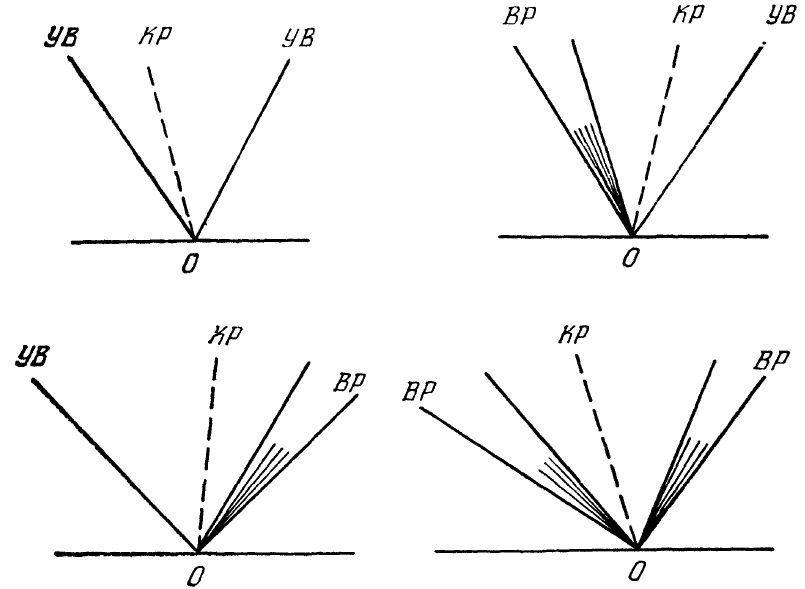
\includegraphics[width=0.9\textwidth]{godunov1976_fig13-1}
	\caption{
		Рисунок из \cite{godunov1976}, иллюстрирующий возможные автомодельные случаи об эволюции разрыва.
	}
	\label{fig:godunov1976_fig13-1}
\end{figure}


%----------------------------
\section{Задача Сода }

Исследуем задачу Сода \cite{sod1978}.

\todo{Запрограммировать аналитическое решение, см цель \url{https://github.com/MathZIVota/Simulation-of-radio-emission-from-supernova-/issues/4}}

\todo{Написать численный решатель этой задачи} 


\clearpage
\sloppy
\printbibliography

%-------------------------------------------------

\ifnum \value{basement}=1

\newpage


\section*{Не используемые картинки}


%
\begin{figure}[!htb]
	\centering
	\includegraphics[width=0.9\textwidth]{spectrum_sn2018aoq_35_day}
	\caption{
		Наблюдаемый спектр сверхновой SN2018aoq
		на 25~апреля~2018 года (35-й день после взрыва) -- синяя линия.
		Соответствующие модельные спектры
		\tardis -- оранжевая линия.
		M1 -- зелёная линия.
	}
	\label{fig:spectrum_sn2018aoq_35_day}
\end{figure}

\fi

\end{document}
